\chapter{Prerequisites and basic notions}

\section{Basics}

We assume that the reader is familiar with the following notions.

\subsection{Algebraic identities}
\begin{itemize}[itemsep=1pt,label=$\circ$]
    \item $(a + b)^2 = a^2 + 2ab + b^2$
    \item $a^2 - b^2 = (a + b)(a - b)$
    \item $a^3 - b^3 = (a - b)(a^2 + ab + b^2)$
    \item $a^3 + b^3 = (a + b)(a^2 - ab + b^2)$
\end{itemize}

\subsection{Exponents}
Let $a, b \in \mathbb{R}$ and $n, m \in \mathbb{N}$.
\begin{itemize}[itemsep=1pt,label=$\circ$]
    \item $a^n \cdot a^m = a^{n+m}$
    \item $a^n \cdot b^n = (ab)^n$
    \item $\frac{a^n}{a^m} = a^{n-m}$
    \item $a^0 = 1$ if $a \neq 0$
    \item $(a^n)^m = a^{n \cdot m}$
    \item $\sqrt[n]{a} = a^{1/n}$
    \item $(\frac{a}{b})^n = \frac{a^n}{b^n}$
    \item $a^1 = a$
\end{itemize}

\subsection{Logarithms}
Let $a, b > 0$, and $c \in \mathbb{R}$.
\begin{itemize}[itemsep=1pt,label=$\circ$]
    \item $\log(ab) = \log(a) + \log(b)$
    \item $\log(\frac{a}{b}) = \log(a) - \log(b)$
    \item $\log(a^c) = c \cdot \log(a)$
    \item $\log(1) = 0$
\end{itemize}

\subsection{Trigonometry}
The functions $\sin(x), \cos(x), \tan(x)$ are defined for $x \in \mathbb{R}$. We have the following identities:

\begin{itemize}[itemsep=1pt,label=$\circ$]
    \item $\tan(x) = \frac{\sin(x)}{\cos(x)}$ if $\cos(x) \neq 0$
    \item $\cot(x) = \frac{\cos(x)}{\sin(x)}$ if $\sin(x) \neq 0$
    \item $\sin(a \pm b) = \sin(a)\cos(b) \pm \cos(a)\sin(b)$
    \item $\cos(a \pm b) = \cos(a)\cos(b) \mp \sin(a)\sin(b)$
\end{itemize}

\section{Functions}
The elementary functions include polynomials, rational functions, algebraic functions, exponential functions and trigonometric functions.

\begin{definition}[Polynomial functions]
    A polynomial is a function of the form $P(x) = a_n x^n + a_{n-1} x^{n-1} + \ldots + a_1 x + a_0$ where $a_i \in \mathbb{R}$ and $n \in \mathbb{N}$.
\end{definition}

\begin{eg}
    Examples of polynomial functions include:
    \begin{itemize}[itemsep=1pt,label=$\circ$]
        \item $P(x) = 2x^3 - 4x + 7$ (cubic polynomial)
        \item $P(x) = x^2 - 5x + 6$ (quadratic polynomial)
        \item $P(x) = 3x + 1$ (linear polynomial)
        \item $P(x) = 5$ (constant polynomial)
    \end{itemize}
\end{eg}

\begin{definition}[Rational functions]
    A rational function is a function of the form $R(x) = \frac{P(x)}{Q(x)}$ where $P(x)$ and $Q(x)$ are polynomials and $Q(x) \neq 0$.
\end{definition}

\begin{eg}
    Examples of rational functions include:
    \begin{itemize}[itemsep=1pt,label=$\circ$]
        \item $R(x) = \frac{x^2 - 1}{x + 2}$
        \item $R(x) = \frac{2x^3 + 3x}{x^2 - 4}$
        \item $R(x) = \frac{1}{x - 5}$
    \end{itemize}
\end{eg}

\begin{definition}[Algebraic functions]
    An algebraic function is a function that can be expressed as the root of a polynomial equation with coefficients that are polynomials.
\end{definition}

\begin{eg}
    Examples of algebraic functions include:
    \begin{itemize}[itemsep=1pt,label=$\circ$]
        \item $f(x) = \sqrt{x^2 + 1}$
        \item $f(x) = \sqrt[3]{x^3 - 2x + 1}$
        \item $f(x) = \frac{\sqrt{x}}{x + 1}$
    \end{itemize}
\end{eg}

\begin{definition}[Transcendental functions]
    A transcendental function is a function that is not algebraic, such as exponential and trigonometric functions.
\end{definition}

\begin{eg}
    Examples of transcendental functions include:
    \begin{itemize}[itemsep=1pt,label=$\circ$]
        \item $f(x) = e^x$ (exponential function)
        \item $f(x) = \sin(x)$ (trigonometric function)
        \item $f(x) = \ln(x)$ (logarithmic function)
    \end{itemize}

    Below is the graph of the $\sin(x)$ and $\cos(x)$ trigonometric functions.
    \begin{center}
        \begin{tikzpicture}
            \draw[domain=-4.5:4.5, smooth, variable=\x,primary] plot    ({\x}, {sin(\x r)}) node[right] {$\sin(x)$};
            \draw[domain=-4.5:4.5, smooth, variable=\x,secondary] plot    ({\x}, {cos(\x r)}) node[right] {$\cos(x)$};

            \draw[->] (-5,0) -- (5,0) node [above] {$x$};
            \draw[->] (0, -1.2) -- (0, 1.2) node[left] {$y$};
        \end{tikzpicture}
    \end{center}
\end{eg}

\subsection{Graphs transformations}
\begin{definition}[Graph transformations]
    Graph transformations involve shifting, stretching, compressing, and reflecting the graphs of functions. The general form of a transformed function can be expressed as:
    \[
    g(x) = a \cdot f(b \cdot (x - c)) + d
    \]
where:
\begin{itemize}[itemsep=1pt,label=$\circ$]
    \item $a$ affects the vertical stretch/compression and reflection.
    \item $b$ affects the horizontal stretch/compression and reflection.
    \item $c$ affects the horizontal shift.
    \item $d$ affects the vertical shift.
\end{itemize}
\end{definition}

\begin{eg}
    Consider the function $f(x) = \sin(x)$. The following transformations illustrate the effects of the parameters:
    \begin{itemize}[itemsep=1pt,label=$\circ$]
        \item $g(x) = 2 \cdot \sin(x)$ (vertical stretch by a factor of 2)
        \item $g(x) = \sin(2x)$ (horizontal compression by a factor of 2)
        \item $g(x) = \sin(x - \frac{\pi}{2})$ (horizontal shift to the right by $\frac{\pi}{2}$)
        \item $g(x) = \sin(x) + 1$ (vertical shift upwards by 1)
    \end{itemize}
\end{eg}

\subsection{Type of functions}
Let $A$ and $B$ be two sets.

\begin{definition}[Domain and image of a function]
    The domain of a function $f: A \to B$ is the set $A$ where for each element of $a \in A$, the function is defined.
    \\
    The image (or codomain) of the function is the set $B$. For every $a \in A$, there exists a unique $b \in B$ such that $f(a) = b$.
\end{definition}

\begin{definition}[Surjective functions]
    A function $f: A \to B$ is surjective (onto) if for every $b \in B$, there exists at least one $a \in A$ such that $f(a) = b$.
\end{definition}

\begin{definition}[Injective functions]
    A function $f: A \to B$ is injective (one-to-one) if for every $b \in B$, there exists at most one $a \in A$ such that $f(a) = b$.
\end{definition}

\begin{definition}[Bijective functions]
    A function $f: A \to B$ is bijective if it is both injective and surjective. This means that for every $b \in B$, there exists exactly one $a \in A$ such that $f(a) = b$.
\end{definition}

\subsection{Inverse functions}
Let $f: A \to B$ be a bijective function.

\begin{definition}[Inverse function]
    The inverse function of $f$, denoted by $f^{-1}: B \to A$, is defined such that for every $b \in B$, $f^{-1}(b) = a$ where $f(a) = b$.
\end{definition}

\begin{eg}
    Consider the function $f(x) = x^2$ defined on $\mathbb{R}$. This function is bijective on $[0, +\infty)$.
    \\
    To find the inverse function, we solve for $x$ in terms of $y$:
    \[
    y = x^2 \implies x = \sqrt{y}
    \]
    Thus, the inverse function is $f^{-1}(y) = \sqrt{y}$. We can plot both functions to visualize their relationship.
    \begin{center}
        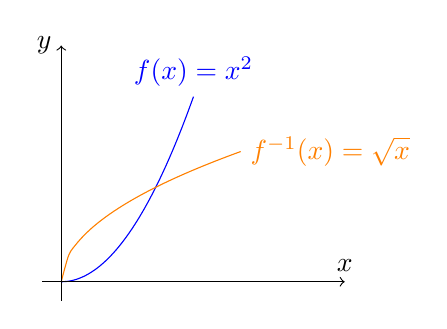
\begin{tikzpicture}[scale=1.2]
            \draw[domain=0:1.4, smooth, variable=\x,blue] plot    ({\x}, {\x^2}) node[above] {$f(x) = x^2$};
            \draw[domain=0:1.9, smooth, variable=\x,orange] plot    ({\x}, {sqrt(\x)}) node[right] {$f^{-1}(x) = \sqrt{x}$};

            \draw[->] (-0.2,0) -- (3,0) node [above] {$x$};
            \draw[->] (0, -0.2) -- (0, 2.5) node[left] {$y$};
        \end{tikzpicture}
    \end{center}
\end{eg}